\documentclass{article}
\usepackage{graphicx}
\usepackage[utf8]{inputenc}
\usepackage[fleqn]{amsmath}
\usepackage{titling}
\usepackage{graphicx,wrapfig,lipsum}
\usepackage{amssymb}
\usepackage{listings}
\usepackage[font=small,labelsep=none]{caption}
\usepackage{array}% http://ctan.org/pkg/array
\usepackage{lipsum}
\usepackage{subcaption}
\usepackage{float}
\usepackage{hyperref}

\setlength{\droptitle}{-10em}

\title{Project 4}\vspace{-3ex}
\author{Benedicte Allum Pedersen, Emil Helland Broll and Fredrik Oftedal Forr}
\date{\vspace{-5ex}}

\begin{document}

\begin{titlepage}
  \centering
  
\includegraphics[width=0.15\textwidth]{./pics/uio.png}\par\vspace{1cm}
  {\scshape\LARGE Universitetet i Oslo\par}
  \vspace{1cm}
  {\scshape\Large Project 5\par}
  \vspace{1.5cm}
  {\huge\bfseries Making a model for the solar system using ordinary differential equations\par}
  \vspace{2cm}
  {\Large\itshape Benedicte Allum Pedersen, Fredrik Oftedal Forr og Emil Helland Broll\par}
	\vfill

  \vfill
  {\large 24. november 2019\par}
\end{titlepage}

\section*{Abstract}

\tableofcontents

\newpage

\section{Introduction}
We have used the velocity Verlet algorithm for solving coupled ordinary differential equations and object orientation for making a model for the soslar system. The equations we have used for this is based on Newton's law of motion due to the gravitational force.

For a hypothetical solar system with only the Earth and the sun Newton's law is given by one force $F_G$

\begin{flalign}
    F_G =\frac{GM_{\odot}M_{Earth}}{r^2}
\end{flalign}

In the above equation $M_{\odot}$ and $M_{Earth}$ is the mass of the Sun and the Earth. G is the gravitational constant and r is the distance between the Earth and the Sun. We neglect the motion of the Sun and only look at the motion of the Earth relative to the Sun. We can do this because we assume that the mass of the Sun is much larger than the mass of the Earth. The gravitiational force consits of a x and y component $F_{G,x}$ and $F_{Gy}$, we then use Newton's second law and obtain:

\begin{flalign}
    \frac{d^2x}{dt^2} = \frac{F_{G,x}}{M_{Earth}} \ \
    \text{and} \ \
    \frac{d^2y}{dt^2} = \frac{F_{G,y}}{M_{Earth}}
\end{flalign}

We use that the average distance bewteen the Earth and the Sun is $1.5 \cdot 10^{11}$ m and we call this one astronomical unit (1 AU). We use the masses of the different planets including the sun that are given in \href{http://compphysics.github.io/ComputationalPhysics/doc/Projects/2019/Project5/SolarSystem/pdf/SolarSystem.pdf}{the description of Project 5}.

\section{Method}
We assume that the orbit of the Earth is circular around the sun, we then have that:

\begin{flalign}
    F_G = \frac{M_{Earth}v^2}r = \frac{GM_{\odot}M_{Earth}}{r^2}
\end{flalign}

We then solve for $v^2r$, where $v$ is the velocity of Earth.

\begin{flalign}
    v^2r = G M_{\odot} = 4\pi^2 \ \ AU^3/(yr)^2
\end{flalign}

where yr is short for years, which we use instead of seconds to decribe the motions in the solar system.


\section{Results}

Euler kræver mang flær steps size enn værlet metoden for å bli nøyaktig

\begin{figure}
    \begin{center}
        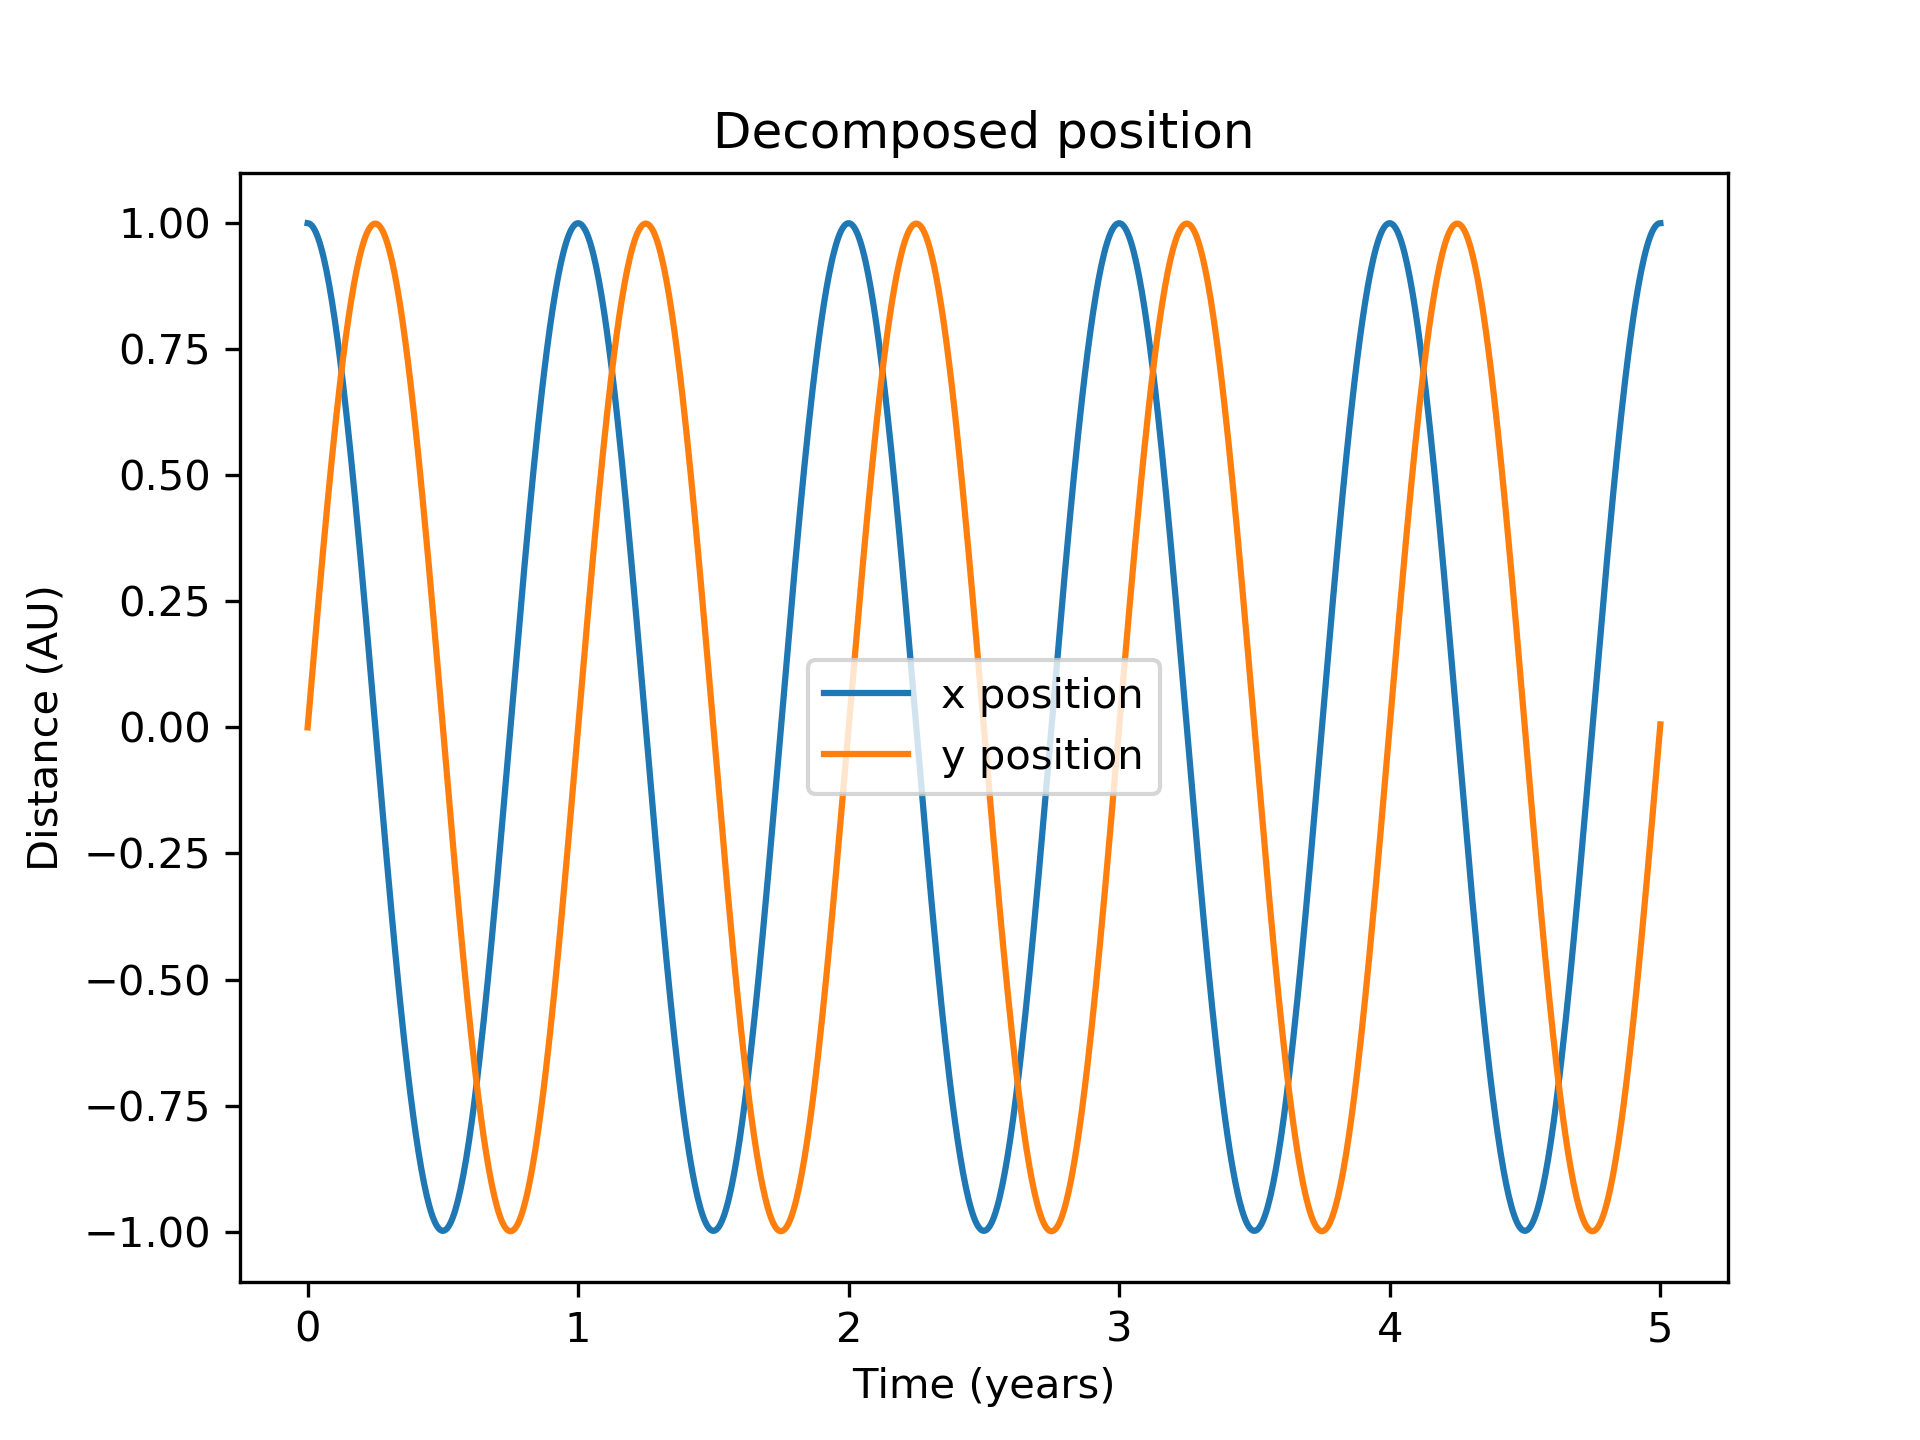
\includegraphics[width=\textwidth]{./Plot/xy_vs_time.png}
        \caption{}
        \label{}
    \end{center}
\end{figure}

\section{Discussion}

\section{Appendix}

\section{Bibliography}

\begin{figure}
    \begin{center}
        \includegraphics[width=\textwidth]{./Plot/}
        \caption{}
        \label{}
    \end{center}
\end{figure}

\end{document}
